\section{Theoretische Grundlagen}
\label{sec:Theorie}
Zuerst betrachten wir wie es zur Dipolen in Ionenkristallen kommt und welche
Eigenschaften diese haben. Dazu betrachte man die Abbildung \ref{theo1}, es ist
ein Ionengitter mit einwertigen Ionen abgebildet (CsJ). Zur Erzeugung
der Dipole wird dieses Gitter mit $\text{Sr}^{2+}$ dotiert. Da der Kristall
elektrisch neutral ist, hat dieses eine Leerstelle zufolge. Es bildet
sich ein Dipol zwischen dem dotierten Ion ($\text{Sr}^{2+})$ und der Leerstelle
mit einer Vorzugrichtung aus. Die so entstehenden Richtungen sind aufgrund
des Kristall diskretisiert.
\begin{figure}
\centering
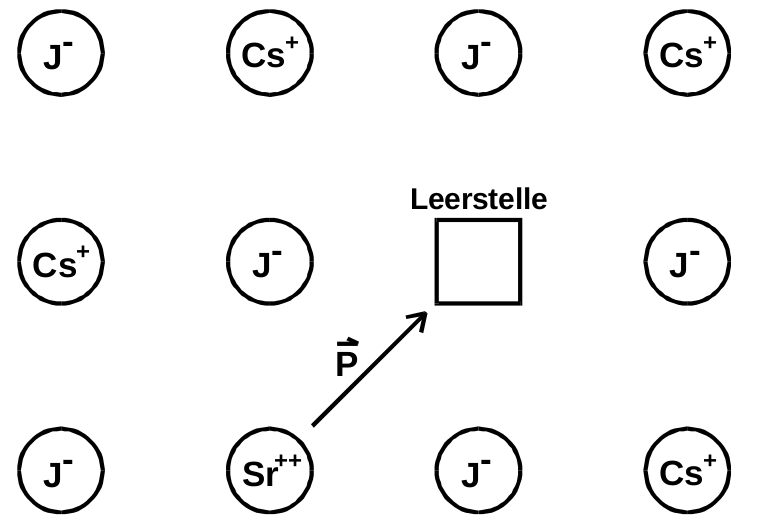
\includegraphics[width=0.8\textwidth]{ressources/ionengitter.png}
\caption{Darstellung eines Ionenkristallgitters mit einem ausgebildeten Dipol. \cite{skript}}
\label{theo1}
\end{figure}
Das Verhalten dieser Dipole hängt von der Temperatur des Kristalls ab. Für
Temperaturen unter $500°$C wird eine Änderung des Dipols nur über eine
Leerstellendiffusion erzeugt.
Diese kann nur statt finden, wenn eine materialspezifische Aktivierungsenergie
aufgebracht werden kann. Diese wird benötigt um die Änderung des Gitterpotentials
,welches durch die neue Konfiguration entsteht, zu ermöglichen. Die mittlere
Zeit die ein Dipol braucht, bis zwei Umorientierungen stattfinden bezeichnet man
als Relaxationszeit. Diese hängt davon ab wie viel des Gesamtdipolmoments die Energie
$W$ besitzt um die Potentialschwelle zu überwinden. Diese Größe ist
Boltzmann verteilt. Die Relaxationszeit ist gegeben durch:


\begin{equation}
    \label{Formel1}
\tau(T)=\tau_0 \exp(\frac{W}{k_\text{B}T})
\end{equation}
Das $\tau_0$ wird als charakteristische Relaxationszeit bezeichnet und
gibt das Verhalten der Relaxationszeit im unendlichen an, sie ist
definiert als $\tau_0=\tau(\infty)$. Nach Definition der zu bestimmenden
Größen wird nun eine Betrachtung des Messverfahren durchgeführt.
\subsection{Messverfahren}
Zur Untersuchung der Dipole wird ein Plattenkondensator mit
Dielektrikum verwendet. Das Dielektrikum besitzt Dipole  die sich
ausrichten können. Hierzu wird ein elektrisches
Feld der Feldstärke $E$ angelegt. Dies führt zur einer Ausrichtung der
Dipole entlang des Feldes. Effekte wie die thermische Bewegungen des Gitters und
ähnliche Effekte führen dazu, dass sich nur ein Bruchteil der Dipole ausrichten kann.
Dieser Bruchteil $y$ lässt sich durch die Langevin-Funktion, welche ein
Funktion zur Berechnung von Orientierungspolarisationen ist, berechnen.
Sie ist gegeben durch:
$$y=L(x)=\coth(x)-1/x$$
Die Langevin-Funktion ist eine allgemeine Funktion, für den hier
betrachteten Fall lässt sich das $x$ identifizieren als
$$x=\frac{pE}{kT}.$$
Für das durchgeführte Experiment kann die Näherung getroffen werden das
$$pE \ll KT$$
sodass sich für die Langevin-Funktion ergibt:
$$y(T)=\frac{pE}{3kT}$$
Zusätzlich muss angenommen werden, dass Dipole sich lange gegenüber der
Relaxationszeit im E-Feld aufhalten. Damit die obenstehende Gleichung
gilt.\\
Es wird nun der Strom betrachtet der entsteht wenn sich die Dipole ausrichten,
dieser ist proportional zum Anteil der bei der Polarisationstemperatur $T_p$
 polarisierten Dipole, zum Probenquerschnitt $F$ und der relaxierenden Dipole $\text{d}N/\text{d}t (t)$.
 Es folgt:
$$ j(T)=y(T_p)F \frac{\text{d}N}{\text{d}t}(T)$$
Der Ausdruck $\frac{\text{d}N}{\text{d}t}(T)$ lässt sich Nähern, sodass gilt:
$$j(T)\approx y(T_p)\frac{F N_p}{\tau_o} \exp{\frac{-W}{k_bT}}$$
$$j(T)\frac{\tau_0}{F_p N_p y(T_p)}\approx \exp{\frac{-W}{k_bT}} $$
Sodass schließlich näherungsweise ein Zusammenhang zwischen der Aktivierungsenergie $W$ herstellen lässt:
\begin{equation}
    \label{Formel5}
    \ln (\frac{j(T)}{1\,\text{A}})+ \ln(\text{const}.)=\frac{-W}{k_bT}
\end{equation}
Alternativ kann man beginnend mit einer Betrachtung der Probenpolarisation
$$ \frac{ \text{d}P}{\text{d}t}= - \frac{P}{\tau (T)}$$
Die Polarisation lässt sich als ein Integral über die Stromdichte darstellen.
$$P(t=\infty)-P(t(T))= \int_{t(T)}^{\infty} j(t')\text{d}t'$$
Der Term $P(t=\infty)$ verschwindet, da nach beliebig langer Zeit alle Dipole
relaxiert sind. Des Weiteren wird erneut die konstante Heizrate $b=\text{d}T/\text{d}t$
angenommen, sodass folgt:
$$ \tau(T)=\int_T^\infty j(T')\text{d}T' \frac{1}{j(T)b}$$
Mit Hilfe der Gleichung \eqref{Formel1} lässt sich $\tau(T)$ ersetzen:
\begin{equation}
    \label{Formel7}
\ln(\int_T^\infty j(T')\text{d}T')-\ln(j(T)\tau_0 b)=\frac{W}{k_BT}
\end{equation}
Für die folgenden Umformungen wird die obere Integralgrenze
des uneigentlichen Integrals auf eine Temperatur gesetzt, bei der der Strom
verschwindet. Zur Berechnung der charakteristischen Relaxationszeit
$\tau_0$ wird das Maximum der Stromdichte gesucht.
$$ \frac{\text{d}j}{\text{d}T}\left|_{T=T_\text{max}} \right.$$
Mit Hilfe des Maximierungsproblems lässt sich die Formel für das $\tau_0$
gewinnen:
\begin{equation}
    \label{Formel8}
    \tau_0=b^{-1}\exp \left(-\frac{W}{k_b T_{\text{max}}}\right)
            \frac{k_BT^2_\text{max}}{W}.
\end{equation}

\begin{figure}
\centering
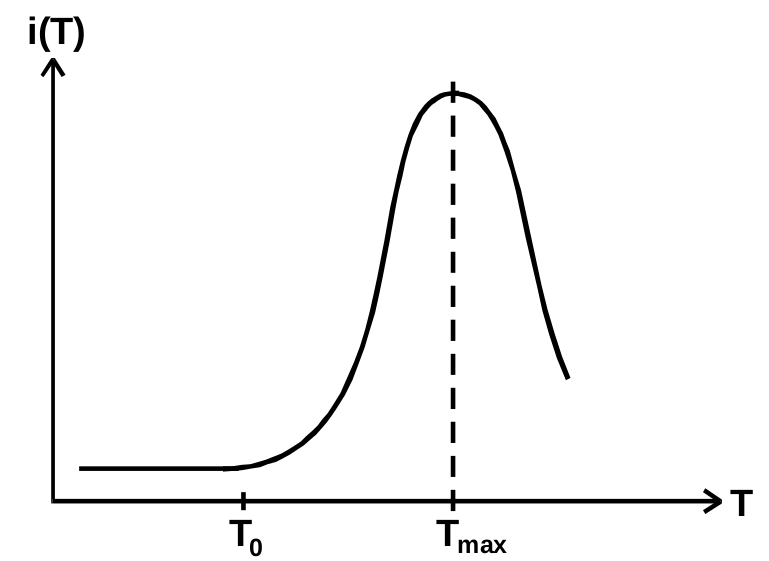
\includegraphics[width=0.8\textwidth]{ressources/stromfluss.png}
\caption{Darstellung des Stromverlaufs bei steigender Temperatur. \cite{skript}}
\label{theo1}
\end{figure}



% 2x2 Plot
% \begin{figure*}
%     \centering
%     \begin{subfigure}[b]{0.475\textwidth}
%         \centering
%         \includegraphics[width=\textwidth]{Abbildungen/Schaltung1.pdf}
%         \caption[]%
%         {{\small Schaltung 1.}}
%         \label{fig:Schaltung1}
%     \end{subfigure}
%     \hfill
%     \begin{subfigure}[b]{0.475\textwidth}
%         \centering
%         \includegraphics[width=\textwidth]{Abbildungen/Schaltung2.pdf}
%         \caption[]%
%         {{\small Schaltung 2.}}
%         \label{fig:Schaltung2}
%     \end{subfigure}
%     \vskip\baselineskip
%     \begin{subfigure}[b]{0.475\textwidth}
%         \centering
%         \includegraphics[width=\textwidth]{Abbildungen/Schaltung4.pdf}    % Zahlen vertauscht ... -.-
%         \caption[]%
%         {{\small Schaltung 3.}}
%         \label{fig:Schaltung3}
%     \end{subfigure}
%     \quad
%     \begin{subfigure}[b]{0.475\textwidth}
%         \centering
%         \includegraphics[width=\textwidth]{Abbildungen/Schaltung3.pdf}
%         \caption[]%
%         {{\small Schaltung 4.}}
%         \label{fig:Schaltung4}
%     \end{subfigure}
%     \caption[]
%     {Ersatzschaltbilder der verschiedenen Teilaufgaben.}
%     \label{fig:Schaltungen}
% \end{figure*}
